\documentclass[10pt,a4paper]{article}
\usepackage[margin=1.9cm,top=1.7cm,bottom=1.8cm]{geometry}
\usepackage[T1]{fontenc}\usepackage{lmodern}\usepackage{textcomp}
\usepackage{graphicx,booktabs,float,amsmath,enumitem,titlesec}
\usepackage[hidelinks]{hyperref}
\graphicspath{{../thesis/}}
\setlength{\parskip}{0.35em}\setlength{\parindent}{0pt}
\titlespacing*{\section}{0pt}{0.9em}{0.25em}
\titleformat{\section}{\large\bfseries}{\thesection}{0.6em}{}
\setlist{nosep,leftmargin=1.4em}
\setlength{\textfloatsep}{6pt}\setlength{\intextsep}{6pt}
\begin{document}
{\small\textsc{Master Thesis Project \textperiodcentered{} Final Evaluation \textperiodcentered{} Short Report \textperiodcentered{} November 2026}}\par\vspace{4pt}
{\LARGE\bfseries A Multi-Agent LLM Framework for Explainable Algorithmic Trading on NSE-Listed Equities\par}\vspace{5pt}
Vipluv (22MF3IM22) \textperiodcentered{} Department of Industrial \& Systems Engineering, IIT Kharagpur \textperiodcentered{} Supervisor: Prof.\ S.\ P.\ Sarmah\par
\vspace{4pt}\hrule\vspace{6pt}

\textbf{Summary.} This project builds and evaluates an explainable multi-agent decision-support system for NSE-listed equities: a technical agent (peephole LSTM with temporal attention), an LLM headline-sentiment agent, a market-regime agent, a point-in-time fundamentals agent, a bull/bear LLM debate and a deterministic risk manager. Every configuration is evaluated on a purged, embargoed walk-forward (19,110 out-of-sample decisions, 2018-12-07 to 2026-08-27) under the full Indian delivery cost schedule (about 32 bps round trip). \textbf{No configuration beats Buy-and-Hold} (net Sharpe 0.59; best agent configuration, Tech+Regime, 0.35). The result replicates on a universe three times larger and on data the mid-semester study never saw. What the system does deliver is risk control and auditability: the regime-aware configurations roughly halve maximum drawdown, and the decision rationales are exactly reconstructable and faithful under deletion tests.

\section{Objective and status}
Most published stock-prediction systems emit a score with no rationale and are validated on US indices with backtests that ignore transaction costs. This project adapts three lines of work to Indian equities (PLSTM-TAL [1], LLM headline sentiment [2], multi-agent debate [3]) and evaluates them under one protocol strict enough that a negative answer is trustworthy. All objectives from the initial and mid-semester reports are complete:
\begin{itemize}
\item \textbf{Mid-semester:} technical, sentiment and regime agents; bull/bear debate; rule-based risk manager; backtest against Buy-and-Hold, MACD, RSI and KDJ+RSI.
\item \textbf{November plan:} larger LLM (Qwen2.5-3B vs 1.5B); extended universe (30 names, data to Nov 2026); sentiment around earnings announcements; point-in-time fundamentals agent; cost-aware position sizing; full ablation re-run; explainability evaluation.
\end{itemize}

\section{Data}
\begin{itemize}
\item \textbf{Prices:} 10 liquid NSE large caps (core, Jan 2015 -- Sep 2026) and 30 Nifty-50 names (extended, to Nov 2026), adjusted daily OHLCV from Yahoo Finance; Nifty 50 and India VIX as benchmarks.
\item \textbf{News:} 34,992 noise-filtered headlines from Indian outlets, 2016 -- Aug 2026. After-close headlines move to the next day, and weekend/holiday dates roll to the next trading session.
\item \textbf{Fundamentals:} annual P\&L and balance sheets for 30 names, FY2015 -- FY2026 (screener.in).
\end{itemize}

\section{Method}
\textbf{Technical agent.} Peephole LSTM cells and a temporal-attention layer, written from scratch in PyTorch, trained on 30-day feature sequences to predict whether the stock rises from the next open to the following open. A $2\times2$ ablation (peephole $\times$ attention), three seeds each; predictions are seed-averaged.

\textbf{Sentiment agent.} Qwen2.5 labels each headline \emph{Good}, \emph{Bad} or \emph{Unknown} by reading the three labels' first-token logits in one forward pass: deterministic and never unparseable. The agent abstains on days without news.

\textbf{Regime agent.} Four causal, equally weighted votes: price vs its 200-day average, 60-day relative strength vs the Nifty, position in the 52-week range, and (optionally) Nifty momentum.

\textbf{Fundamentals agent (new).} Uses only annual statements, each hidden until 61 days after the fiscal year end (one day past the SEBI LODR Regulation 33 deadline), so it can be late but never early. Net-profit growth, revenue growth, ROE and change in ROE are z-scored across the universe on each decision date.

\textbf{Debate.} On contested days a bull and a bear researcher argue from the agents' findings; the LLM scores each case and the residual moves the score by a fixed 35\% weight. The mid-semester gate escalated 97.4\% of days; the conviction gate used in the final run escalated 10.5\% of decisions without the fundamentals agent and 28.9\% with it.

\textbf{Trader and risk manager.} A confidence-weighted mean of stances, then a deterministic risk manager: confidence floor, 20\% volatility target, drawdown brake, 20\% per-name cap and 100\% gross cap; idle cash earns 6\%. Two cost-aware components are new and opt-in: an \emph{edge-vs-cost gate} (trade only if expected edge exceeds round-trip cost) and a \emph{no-trade band} of 0.05 (held positions are not resized inside the band; entries and exits are never banded).

\textbf{Evaluation protocol.} Purged, embargoed walk-forward: 3-year training windows, 6-month test windows, 10-day embargo, 16 folds. Decisions at the close of day $t$ execute at the open of $t+1$. Costs follow the 2026 delivery schedule (STT, stamp duty, exchange and SEBI charges with GST, 5 bps slippage). Sharpe ratios are excess of 6\% with block-bootstrap 95\% CIs; differences vs Buy-and-Hold are Holm-corrected across all configurations.

\section{Results}
\textbf{Technical agent: at chance.} No architecture is distinguishable from a coin flip on the core universe (LSTM 0.5045, LSTM-TAL 0.5024, PLSTM-TAL 0.4998, PLSTM 0.4996; all $p$ vs chance $\geq 0.21$). Re-trained on 30 names (58,620 out-of-sample rows per run) the result is the same: LSTM-TAL 0.4999, PLSTM-TAL 0.4987.

\textbf{Core ablation.} All configurations share the same 19,110 decisions, execution and cost model (Table~\ref{tab:core}, Figure~\ref{fig:eq}).

\begin{table}[H]
\centering\small
\caption{Core ablation (10 names), selected rows. Sharpe is net of costs and excess of 6\% risk-free.}\label{tab:core}
\resizebox{\linewidth}{!}{%
\begin{tabular}{lrrrrrrr}
\toprule
\textbf{Strategy} & \textbf{Sharpe net} & \textbf{Sharpe gross} & \textbf{CAGR} & \textbf{MaxDD} & \textbf{Turnover/yr} & \textbf{Exposure} & \textbf{Holm p} \\
\midrule
Buy\&Hold & 0.59 & 0.59 & 16.4\% & -38.6\% & 0.1x & 100\% & -- \\
RSI(14) & 0.43 & 0.47 & 12.3\% & -39.8\% & 4.2x & 60\% & 0.818 \\
Tech+Regime & 0.35 & 0.58 & 10.1\% & -20.7\% & 20.4x & 86\% & 0.818 \\
Regime+Fund+Band & 0.28 & 0.47 & 9.0\% & -22.2\% & 16.0x & 84\% & 0.598 \\
Tech+Regime+Fund & 0.24 & 0.50 & 8.5\% & -23.2\% & 23.2x & 88\% & 0.588 \\
Regime+Fund & 0.21 & 0.48 & 8.2\% & -23.2\% & 23.6x & 88\% & 0.588 \\
Tech+Sent+Regime & 0.17 & 0.66 & 7.5\% & -25.0\% & 43.4x & 90\% & 0.414 \\
All4+Debate(conviction) & 0.14 & 0.60 & 7.0\% & -24.7\% & 43.1x & 93\% & 0.088 \\
Tech+Regime+Fund+CostAware+Band & 0.14 & 0.37 & 6.5\% & -5.3\% & 5.2x & 7\% & 0.818 \\
MACD & 0.02 & 0.46 & 5.0\% & -29.9\% & 42.9x & 78\% & 0.387 \\
Tech-only & -0.41 & -0.27 & 3.1\% & -25.4\% & 5.5x & 16\% & 0.088 \\
MeanReversion & -1.41 & 0.68 & -18.1\% & -79.6\% & 223.4x & 76\% & 0.000 \\
\bottomrule
\end{tabular}}
\end{table}

\begin{figure}[H]
\centering
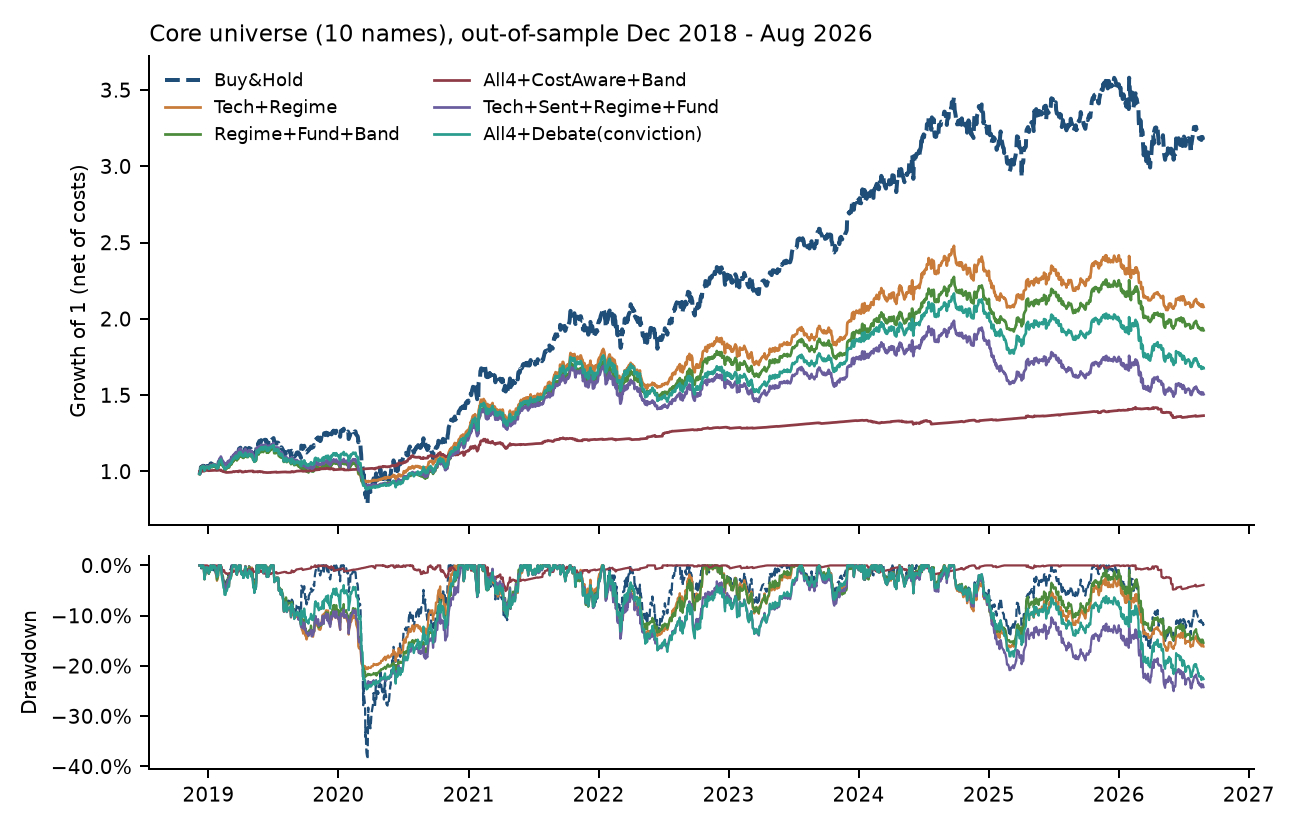
\includegraphics[width=0.78\linewidth]{equity_core.png}
\caption{Equity and drawdown, core universe, net of costs.}\label{fig:eq}
\end{figure}

\textbf{What each new component did.}
\begin{itemize}
\item \textbf{Fundamentals} lower Sharpe when added to Tech+Regime (0.35 $\to$ 0.24) and do not rescue the sentiment configuration (0.17 $\to$ 0.04).
\item \textbf{The no-trade band} cuts turnover (23.6x $\to$ 16.0x a year) and lifts Sharpe (0.21 $\to$ 0.28): the only component that helps, and it helps by trading less, not by predicting better.
\item \textbf{The edge-vs-cost gate} exposes the core finding: almost no signal clears the 32 bps hurdle, so the book is invested only 7\% of the time. Its small drawdown is the drawdown of cash.
\item \textbf{Conviction-gated debate:} 0.14 without fundamentals, 0.14 with them.
\end{itemize}

\textbf{Extended universe.} The technical agent is re-trained on 30 names and run to 2026-11-04 (58,620 decisions). No news corpus exists for the 20 added names, so this tests the technical, regime and fundamentals agents and the risk layer (Table~\ref{tab:ext}). The ordering replicates, and with three times the cross-section the negative result sharpens: four agent configurations are now \emph{significantly worse} than Buy-and-Hold after Holm correction. On the fresh Sep--Nov 2026 holdout (44 days, too short for inference) Buy-and-Hold returned 3.15\% against $-2.49\%$ for Tech+Regime.

\begin{table}[H]
\centering\small
\caption{Extended universe (30 names), selected rows. Same protocol and costs.}\label{tab:ext}
\begin{tabular}{lrrrrrr}
\toprule
\textbf{Strategy} & \textbf{Sharpe net} & \textbf{Sharpe gross} & \textbf{CAGR} & \textbf{MaxDD} & \textbf{Turnover/yr} & \textbf{Holm p} \\
\midrule
Buy\&Hold & 0.74 & 0.74 & 18.5\% & -34.3\% & 0.1x & -- \\
RSI(14) & 0.66 & 0.74 & 17.5\% & -38.5\% & 9.3x & 0.558 \\
Regime+Fund+Band & 0.36 & 0.57 & 10.2\% & -25.1\% & 16.3x & 0.038 \\
Tech+Regime & 0.35 & 0.67 & 10.4\% & -24.7\% & 29.1x & 0.031 \\
Tech+Regime+Fund & 0.25 & 0.57 & 8.8\% & -27.8\% & 28.9x & 0.006 \\
Regime+Fund & 0.25 & 0.56 & 8.7\% & -27.8\% & 29.0x & 0.006 \\
MACD & 0.23 & 0.91 & 8.5\% & -29.1\% & 70.1x & 0.086 \\
Tech-only & 0.09 & 0.29 & 6.4\% & -7.7\% & 7.2x & 0.198 \\
\bottomrule
\end{tabular}
\end{table}

\textbf{Sentiment, earnings and model size.} On the full corpus, debiased daily sentiment predicts neither the next day nor the next five (every information coefficient indistinguishable from zero, Holm $p=1.000$). Both LLMs then scored an identical 10,240-headline matched sample. They agree on 60.3\% of labels (Cohen's $\kappa=0.39$); the 3B model is far less bullish (Good:Bad 1.70 against 3.14) and says \emph{Unknown} far more often (68.5\% vs 34.3\%). On earnings sessions the raw tone predicts the next open-to-open return with the \emph{opposite} sign for both models (IC $-0.084$ and $-0.085$; Holm $p$ 0.003 and 0.002): a reversal, not a continuation. It is not a tradable edge: it does not survive the causal debiasing step (Holm $p$ 0.072), and the spread ($-26$ and $-37$ bps) is of the same order as the 32 bps round-trip cost. A larger model changes how headlines are labelled, not the conclusion.

\textbf{Risk control in stressed markets.} Over crash-regime days (Nifty trailing 60-day return below $-10\%$; 94 days, almost all in the 2020 COVID crash) the regime-aware configurations protect capital: maximum drawdown is $-1.1\%$ for Tech+Regime, $-2.5\%$ for Regime+Fund and $-8.8\%$ for All4+Debate(conviction), against $-23.6\%$ for Buy-and-Hold. The overlay trades upside for downside protection, and over the full period that trade loses on net.

\section{Explainability}
Explainability is treated as a testable property. Four checks run over every logged decision: \emph{provenance} (does the rationale name the model that produced its numbers?), \emph{integrity} (do stated values equal logged values?), \emph{reconstruction} (can the score be recomputed from the logged opinions?) and \emph{deletion faithfulness} (does removing the top-attributed agent flip the decision more often than removing another?).
\begin{itemize}
\item \textbf{Integrity and reconstruction} pass at 100.00\% on every decision log, mid-semester and final.
\item \textbf{Provenance found a real defect:} all 19,110 mid-semester rationales credited PLSTM-TAL for predictions produced by LSTM-TAL. Every number was correct; the explanation was not. It is fixed, and the final logs pass at 100\%.
\item \textbf{Deletion faithfulness} (Table~\ref{tab:del}): removing the top-attributed agent flips 37.4--71.3\% of decisions, against 0.0--3.4\% for another agent (McNemar $p<10^{-6}$ in every configuration).
\end{itemize}

\begin{table}[H]
\centering\small
\caption{Deletion faithfulness, selected configurations.}\label{tab:del}
\begin{tabular}{lrrr}
\toprule
\textbf{Configuration} & \textbf{n} & \textbf{Flip: delete top agent} & \textbf{Flip: delete other agent} \\
\midrule
Tech+Regime & 19,080 & 71.3\% & 0.0\% \\
Full+Debate(conviction) & 19,102 & 52.7\% & 0.5\% \\
Tech+Regime+Fund & 19,110 & 47.3\% & 2.1\% \\
Regime+Fund+Band & 19,080 & 46.8\% & 3.2\% \\
All4+Debate(conviction) & 19,110 & 37.4\% & 3.4\% \\
\bottomrule
\end{tabular}
\end{table}

\begin{figure}[H]
\centering
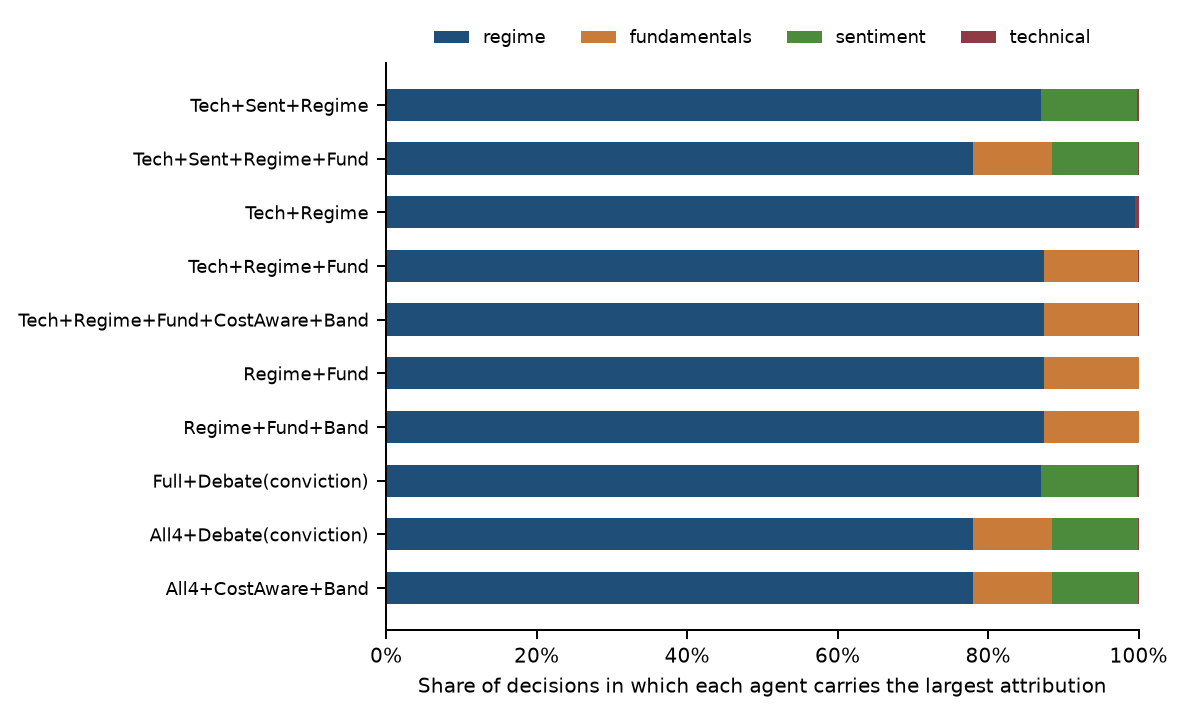
\includegraphics[width=0.78\linewidth]{decisive_agent.png}
\caption{Which agent carries the largest attribution in each decision.}
\end{figure}

The attributions show that the regime agent is the decisive input in the large majority of decisions and the technical model almost never: the system behaves as a trend filter with a risk overlay, which is why it protects capital in crashes and gives up return in rallies. \textbf{There is no accuracy--explainability trade-off here:} black-box models (0.4996--0.5045 directional accuracy, explainability score 0 of 5) and explainable configurations (0.5006--0.5055, score 4--5) all sit at chance, so the explainable design is preferable at no cost.

\section{Limitations}
\begin{itemize}
\item \textbf{Statistical power:} the test reliably detects a Sharpe difference of about 1.0 over this window, not smaller; ``no significant difference'' is not ``proven identical''.
\item \textbf{Model scale:} the comparison is 1.5B vs 3B open models; no hosted frontier model was available.
\item \textbf{Survivorship:} both universes are today's large caps, which flatters Buy-and-Hold more than the agents.
\item \textbf{Fundamentals and news:} restated annual figures with no valuation ratio; headlines for ten names only.
\end{itemize}

\section{Conclusion}
The system is built, tested and reproducible end to end. Under realistic Indian costs and honest statistics it does not beat Buy-and-Hold: on the original universe, on three times as many stocks, or on data that did not exist at the mid-semester review. None of the November additions changes that. What survives is a regime-aware risk overlay that roughly halves drawdowns, and an explanation layer that is measurably faithful and was itself the instrument that diagnosed why the system behaves as it does. \textbf{Future work:} intraday or event-time horizons; point-in-time vendor fundamentals with valuation ratios; a frontier LLM for the debate; a cross-sectional, market-neutral formulation.

\vspace{4pt}{\footnotesize
\textbf{References.} [1] Latif et al., PLSTM-TAL, \emph{Heliyon} 10(6):e27747, 2024. [2] Lopez-Lira and Tang, Can ChatGPT forecast stock price movements?, arXiv:2304.07619, 2023. [3] Xiao et al., TradingAgents, arXiv:2412.20138, 2024.\par
\textbf{Demo:} \texttt{vipluv01.github.io/nse-multi-agent-trading} \textperiodcentered{} \textbf{Code:} \texttt{github.com/Vipluv01/nse-multi-agent-trading}\par}
\end{document}
